\chapter{Using the PyCharm IDE}

\setcounter{problem}{1}

\section{Get and install}

\begin{fullwidth}

https://www.jetbrains.com/pycharm/download/

\section{Why an IDE?}

As I help students poke around in the pycharm development environment, I often notice that many treat it like a text editor. For example, you copy code out of your Python script and paste it into a console in order to run your programs.  Don't do that. 

Development environments like the one we're using in this class are the culmination of decades of experimentation into making programmers as productive as possible. Using it as a text editor is silly because you might as well just use a text editor, right? There's no point in installing some massive development environment on your machine. There are plenty of good text editors and you are free to use them. A bit of history will help use the development environment productively.

In the bad old days, programmers literally had to flip switches on the front of the machine to insert a boot  program so the machine would actually come up. Then we had punchcards. Then we had line oriented editors like ``edit line 34.''  Yes, my life was that bad in 1980. Tedious but better than physical punch cards. Then we got visual editors where we used cursor keys to move around (enter vi, emacs etc...). We would edit code, exit the editor, and then run our program. A text editor does absolutely nothing for you except let you edit characters in the program.

A development environment {\bf has} a text editor built-in but it knows that you are typing in Python code. Hence you will see that it identifies errors in your code such as syntax errors and often type errors before you even run the program. You don't cut and paste the code into a console somewhere, you just say ``run this program.'' The console is for playing around and experimentation, not testing your program. As the programs get bigger, there's just no way to use the console.  Some of the good stuff with an IDE:

\begin{itemize}
\item The development environment can jump to the definition of a function, even if it's in a built-in library.
\item  You can rename variables and functions using knowledge of Python syntax rather than brain-dead string replace, which could introduce errors. Re-factoring is one of the critical tasks of a programmer.
\item  You can select code and say {\em extract method}. You can select an expression and say {\em introduce variable} etc. 
\item  The development environment knows how to reformat your code. 
\item  When you get a runtime error, you can click on it to go that point in the file that crashed.
\end{itemize}

Most importantly the development environment has a debugger where you can single step through your program to see variables change and understand what has gone wrong.

The development environment helps you understand your program as a whole, particularly when the program spans multiple files. As the programs get bigger, you will find the development environment to be very helpful. Part of my job in this class is to give you good programming habits to prepare you for the coming year and your future jobs.

\section{Give it a test drive}

\noindent Create a sample project, making sure that you are using the latest interpreter from homebrew installation ({\tt /usr/local/Cellar/...}):

\scalebox{.75}{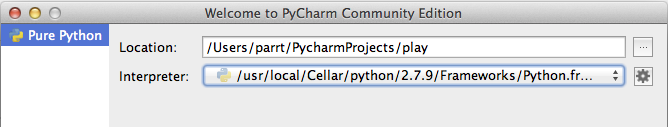
\includegraphics{figures/pycharm-new-project.png}}

\noindent Create a new file with a simple function and run it:

\scalebox{.75}{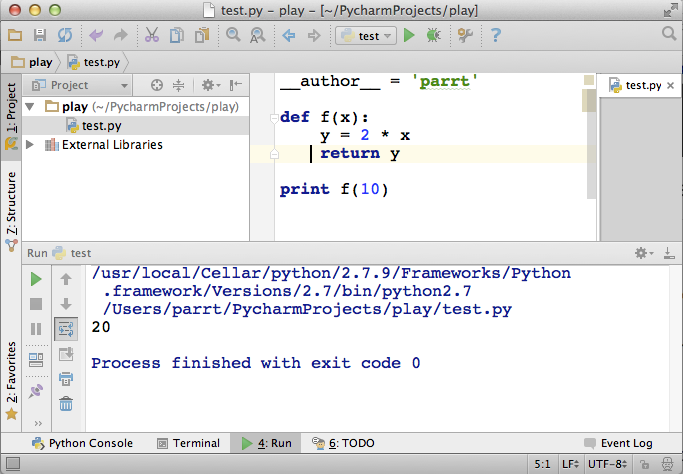
\includegraphics{figures/pycharm-new-file.png}}

\noindent Start up the debugger by clicking the bug icon in the toolbar:

\scalebox{.75}{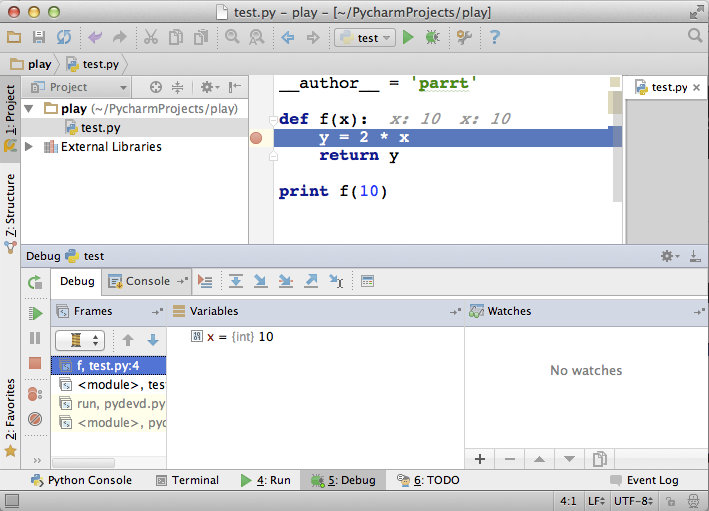
\includegraphics{figures/pycharm-new-dbg.png}}

\noindent Now single step to the next statement:

\scalebox{.75}{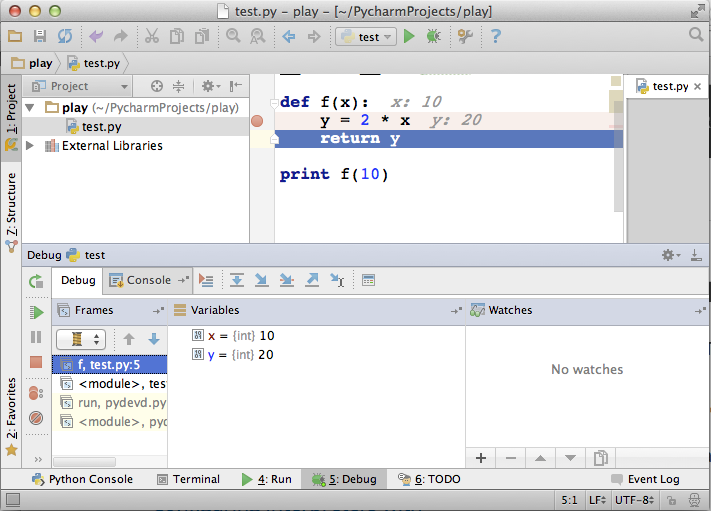
\includegraphics{figures/pycharm-new-dbg2.png}}

\end{fullwidth}
